\chapter{PDE solver}

The program has been run twenty times using a different number of processors each time. The results are listed in the table below:

\begin{center}
\begin{tabular}{|c|c|}
\hline
Numbers of processors & Time to complete \\
\hline
1 & 51.8073 \\
2 & 28.1724 \\
4 & 15.9394 \\
6 & 11.5323 \\
8 & 9.6533 \\
10 & 7.35941 \\
15 & 5.14445 \\
16 & 4.5774 \\
20 & 4.25137 \\ 
24 & 3.20059 \\ 
28 & 3.30171 \\
30 & 3.08664 \\
32 & 2.75156 \\
35 & 2.47561 \\
40 & 2.24806 \\
42 & 2.20288 \\
48 & 1.90164 \\
53 & 1.58522 \\
59 & 1.46382 \\
64 & 1.52331 \\
\hline
\end{tabular}
\end{center}

Using those data, it is possible to compute the \textit{speedup}. The picture \ref{graph} shows it.

\begin{figure}[!h]
\begin{center}
	\includegraphics[width=\textwidth]{pic/graph.ps}
	\caption{Speedup graph}
	\label{graph}
\end{center}
\end{figure}

When we double the number of processors allocated to the program, we could expect that it will only need half of the time it needed previously. As we can see on the graphic, this is not true. Indeed, using 64 processors is only about 34 times faster than using one processor where we could have expected a program 64 times faster. 

The problem is the more processors we use the more communications we do. Those communications introduce a lot of overheads. So, a part of the time won by having a new processor working on the program is spent setting the communications and doing some others things that must be done but does not produce a useful result. This is why the speedup is not what we could have expected.
 
